% Insertable section for Draft 3; requires amsmath, amssymb, amsthm, booktabs,
% tabularx, tikz (arrows.meta,positioning), and theorem/proposition/remark environments.
\section{The geometry, topology, and Borel structure of the representation spectrum}\label{sec:spectral-geometry}
The admissible, unitary, and tempered duals of $G=\mathrm{SL}_2(F)$ encode different kinds of spectral information. This section makes their relationship explicit in rank one. We assume that $F$ is a finite extension of $\mathbb Q_p$, with $p>2$, residue cardinality $q$, valuation $v$, uniformizer $\varpi$, and ring of integers $\mathcal O$. The absolute value is $|a|=q^{-v(a)}$. Our main example is the unramified principal series. Its exceptional fibers explain why the Bernstein variety alone cannot parameterize the trace transform.

\subsection{Four structures on the spectrum}\label{subsec:four-structures}
Write $\widehat G_{\rm ad}$ for the irreducible smooth admissible dual, $\widehat G_u$ for the irreducible unitary dual (identified with its smooth vectors), and $\widehat G_{\rm temp}$ for the tempered dual. We have inclusions
\[\widehat G_{\rm temp}\subseteq\widehat G_u\subseteq\widehat G_{\rm ad}.\]
The following structures answer different questions.
\begin{center}\small
\begin{tabularx}{\linewidth}{@{}p{.23\linewidth}XX@{}}\toprule
Structure & Purpose & Information retained\\\midrule
Standard Borel structure & Direct integrals and measurable representation theory & Measurable sets of irreducibles\\
Fell topology & Convergence and weak containment & Limits of unitary representations\\
Bernstein variety & Algebraic organization of supercuspidal support & Regular dependence on unramified twists\\
Extended quotient & Enhanced spectral parameters & Extra labels at exceptional parameters\\\bottomrule
\end{tabularx}\end{center}
A standard Borel space is a measurable space isomorphic to a Borel subset of a Polish space. It need not be uncountable or isomorphic to the real line. The Fell topology is a topology on the unitary dual, not on arbitrary nonunitarizable smooth representations. The Bernstein variety is an algebraic variety, component by component, and is not generally the space of irreducibles itself. In the unramified block, for instance, the trivial and Steinberg representations have identical supercuspidal support but different temperedness properties.

\subsection{Supercuspidal support and exceptional fibers}\label{subsec:exceptional-fibers}
Let $B=AN$ be the upper triangular Borel subgroup, with $A=\{a(t)=\operatorname{diag}(t,t^{-1}):t\in F^\times\}$. Write $I(\chi)=\operatorname{Ind}_B^G(\chi)$ for normalized smooth induction; the transformation law includes $\delta_B(a(t))^{1/2}=|t|$. Fix a smooth character $\xi$ of $\mathcal O^\times$. The characters extending it are
\[\chi_{\xi,z}(\varpi^n a)=z^n\xi(a),\qquad z\in\mathbb C^\times.\]
The Weyl involution acts by $(\xi,z)\mapsto(\xi^{-1},z^{-1})$. Inertial equivalence identifies supercuspidal pairs up to conjugacy and unramified twist. The Bernstein variety of the corresponding component is $X_{\mathfrak s}=T_{\mathfrak s}/W_{\mathfrak s}$, where $T_{\mathfrak s}$ is the twist torus and $W_{\mathfrak s}$ preserves the inertial class of the inducing character. The support map $\beta:\widehat G_{\rm ad}^{\mathfrak s}\to X_{\mathfrak s}$ records the Weyl orbit of the actual inducing character, not just its restriction to units.

For the unramified block ($\xi=1$), $T_{\mathfrak s}=\mathbb C^\times$ and $W_{\mathfrak s}=\{1,w\}$ with $wz=z^{-1}$. The coordinate $u=z+z^{-1}$ identifies the quotient with $\mathbb A^1_{\mathbb C}$. Indeed $z^n+z^{-n}$ satisfies the recurrence $P_{n+1}=uP_n-P_{n-1}$ with $P_0=2$, $P_1=u$. Thus $\mathbb C[z,z^{-1}]^W=\mathbb C[u]$.

We use the classical rank-one reducibility and unitarity classification as input (see \cite{SS68,Ta92}; precise source checks remain in the verification note). With this normalization, $I(\chi)$ is reducible precisely for $\chi=|\cdot|^{\pm1}$ or nontrivial quadratic $\chi$. The former have the trivial and Steinberg representations as composition factors, each with multiplicity one. The latter split into two inequivalent tempered constituents. In particular $I(1)$ is irreducible. These statements concern smooth induction, not a choice of Hilbert norm at a nonunitary inducing parameter.
\begin{center}\small
\begin{tabularx}{\linewidth}{@{}lllX@{}}\toprule
$z$ & $u$ & Fiber size & Irreducibles\\\midrule
Generic & Generic & 1 & Principal series\\
$1$ & $2$ & 1 & $I(1)$\\
$-1$ & $-2$ & 2 & $\pi_+,\pi_-$ (tempered)\\
$q,q^{-1}$ & $q+q^{-1}$ & 2 & $\mathbf 1,\mathrm{St}$\\\bottomrule
\end{tabularx}\end{center}
Thus the support map has two doubled fibers. The Bernstein center acts by the same scalar on the two members of either fiber, whereas a trace functional can distinguish them.
\begin{figure}[htbp]\centering
\begin{tikzpicture}[>=Latex,x=1cm,y=1cm,every node/.style={font=\small}]
\node[anchor=west] at (0,3.4) {Admissible spectrum (real slice)};
\draw[gray] (.3,2.25)--(11,2.25);
\foreach \x/\lab in {1/{\pi_+},6/{I(1)},9/{\mathbf1}} {\fill (\x,2.25) circle(2pt);\node[below] at (\x,2.25) {$\lab$};}
\fill (1,2.95) circle(2pt) node[right] {$\pi_-$};
\fill (9,2.95) circle(2pt) node[right] {$\mathrm{St}$};
\draw[gray,dashed] (1,2.95)--(1,2.25);\draw[gray,dashed] (9,2.95)--(9,2.25);
\foreach \x in {1,6,9} {\draw[->,dashed] (\x,1.7)--(\x,.6);}
\node at (5,1.15) {$\beta$};
\draw[->] (.3,.45)--(11,.45);
\foreach \x/\lab in {1/{-2},6/{2},9/{10/3}} {\fill (\x,.45) circle(2pt) node[below] {$\lab$};}
\node[anchor=west] at (0,-.35) {Bernstein variety (real slice)};
\end{tikzpicture}
\caption{Support fibers for $F=\mathbb Q_3$. The drawing records fiber cardinalities, not the Fell topology or the entire complex variety.}\label{fig:bernstein-fibers}
\end{figure}

\subsection{The three types of principal-series components}\label{subsec:three-types}
The restriction to units determines which Weyl elements preserve the inertial class. Consequently the classification reduces to three cases.
\begin{center}\small
\begin{tabularx}{\linewidth}{@{}llXX@{}}\toprule
Type & Condition & Variety & Doubled fibers\\\midrule
I & $\xi^2\ne1$ & $\mathbb C^\times$ & None\\
II & $\xi^2=1,\ \xi\ne1$ & $\mathbb C^\times/W$ & $z=\pm1$\\
III & $\xi=1$ & $\mathbb C^\times/W$ & $z=-1$, $\{q,q^{-1}\}$\\\bottomrule
\end{tabularx}\end{center}
In Type I the Weyl involution exchanges the two different unit-character families, so choosing one representative gives the entire twist torus without a further quotient. There are no reducibility points and the unitary and tempered parameters form a circle. In Type II the two quadratic extensions of $\xi$ give two split principal series. The unitary and tempered parameters are a closed interval with both endpoints replaced by two points. In Type III the complementary series $I(|\cdot|^s)$, $0<s<1$, and the trivial representation supplement the tempered spectrum. The Steinberg representation is tempered. These descriptions are set-theoretic until the topology is considered below.

For $p>2$, $F^\times/(F^\times)^2$ has four elements. The Hilbert symbol gives the quadratic characters $\eta_d(t)=(t,d)_F$. Over $\mathbb Q_3$ the nontrivial square classes are $2,3,6$; over $\mathbb Q_5$ they are $2,5,10$. In both examples $\eta_2$ is unramified, and the other two are ramified. For instance $(3,3)_3=-1$, whereas $(5,5)_5=1$. These follow from $(p,p)_p=(-1)^{(p-1)/2}$. Each field has three nontrivial quadratic inducing characters and hence six irreducible tempered constituents in the corresponding exceptional fibers. A ramified quadratic unit character and the trivial unit character therefore supply all three quadratic reducibility parameters.

\subsection{The Fell topology and doubled endpoints}\label{subsec:fell-model}
For unitary representations the Fell topology records weak containment. We use the equivalent topology on the irreducible spectrum of $C^*(G)$, with basic norm-open sets $\{\pi:\|\pi(a)\|>c\}$ for $a\in C^*(G)$ and $c\ge0$. In the unitary principal series $z=e^{i\theta}$, the support coordinate is $u=2\cos\theta$. The complementary series has $u=q^s+q^{-s}$, $0<s<1$. The expected topology in Type III is an interval $[-2,q+q^{-1}]$ with each endpoint doubled. The two copies of each endpoint are distinct but have every neighborhood meeting the same adjacent interval.

\begin{proposition}[Fell convergence from finite-rank traces]\label{prop:fell-trace}
Suppose $\pi_j$ are irreducible unitary representations and $\tau_1,\ldots,\tau_m$ are irreducible unitary representations. Assume that for each $h\in C_c^\infty(G)$,
\[\operatorname{tr}\pi_j(h)\longrightarrow\sum_{i=1}^m\operatorname{tr}\tau_i(h),\]
and that for every compact open subgroup $J$ the dimensions $\dim\pi_j^J$ are uniformly bounded (eventually in $j$). Then $\pi_j\to\tau_i$ in the Fell topology for each $i$.
\end{proposition}
\begin{proof}
Fix $i$ and a basic neighborhood $\|\tau_i(a)\|>c$. Approximate $a$ in the full $C^*$ norm by $h\in C_c^\infty(G)$ so closely that $\|\tau_i(h)\|>c+\epsilon$ and $\|a-h\|<\epsilon$ for some $\epsilon>0$. Choose $J$ so that $h$ is $J$-bi-invariant. For a positive integer $n$, the element $b_n=(h^**h)^{*n}$ (convolution power) is $J$-bi-invariant. Its image is positive, has rank at most $\dim\pi_j^J\le D$, and satisfies
\[D\|\pi_j(h)\|^{2n}\ge\operatorname{tr}\pi_j(b_n)\longrightarrow\sum_k\operatorname{tr}\tau_k(b_n)\ge\|\tau_i(h)\|^{2n}.\]
Here the final inequality holds because the positive operator on the finite-dimensional fixed-vector space has its norm as an eigenvalue. Taking $n$ large enough and then $j$ sufficiently far along the net gives $\|\pi_j(h)\|>c+\epsilon$ (reduce $\epsilon$ first if needed). The norm approximation gives $\|\pi_j(a)\|>c$. Finite intersections of these neighborhoods yield convergence.
\end{proof}

\begin{proposition}[Endpoint limits]\label{prop:endpoint-limits}
Subject to the rank-one classification above, a net of generic unitary principal-series parameters approaching a nontrivial quadratic parameter converges in the Fell topology to both constituents. A net of complementary-series parameters $s\to1$ converges to both $\mathbf1$ and $\mathrm{St}$ in the full unitary dual.
\end{proposition}
\begin{proof}
In the compact picture, $I(\chi_{\xi,z})|_K$, for $K=\mathrm{SL}_2(\mathcal O)$, is independent of $z$. For any compact open $J$, replace it by $J\cap K$ to obtain a uniform bound for the fixed-vector dimensions. For $h$ compactly supported and bi-invariant under a compact open subgroup of $K$, the trace is a Laurent polynomial in $z$: on the finite-dimensional fixed-vector space the Iwasawa decomposition introduces only finitely many valuation powers on the compact support. Therefore the trace converges to the trace of the entire induced module at the limiting parameter. Trace additivity for its finite composition series gives the sum of the two endpoint traces. All representations in that sum are unitarizable. Proposition~\ref{prop:fell-trace} applies. This argument does not require continuity of the complementary-series Hilbert inner products at the endpoint.
\end{proof}

\begin{figure}[htbp]\centering
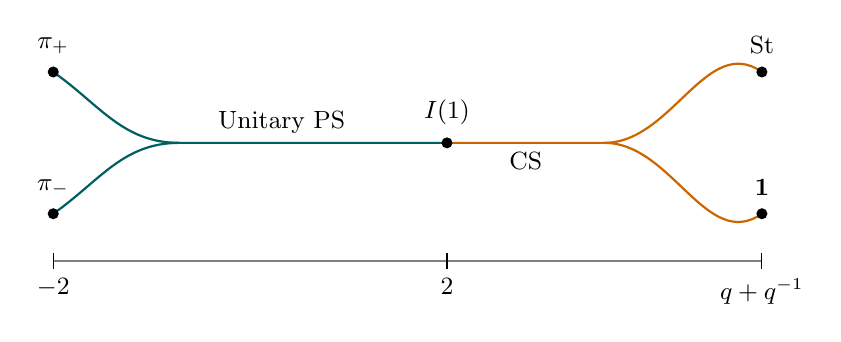
\begin{tikzpicture}[x=1cm,y=1cm,every node/.style={font=\small}]
\draw[teal!75!black,thick] (1,2.6) to[out=-35,in=180] (2.6,1.7)--(6,1.7);
\draw[teal!75!black,thick] (1,.8) to[out=35,in=180] (2.6,1.7);
\draw[orange!80!black,thick] (6,1.7)--(8,1.7) to[out=0,in=145] (10,2.6);
\draw[orange!80!black,thick] (8,1.7) to[out=0,in=-145] (10,.8);
\foreach \x/\y/\lab in {1/2.6/{\pi_+},1/.8/{\pi_-},6/1.7/{I(1)},10/2.6/{\mathrm{St}},10/.8/{\mathbf1}} {\fill (\x,\y) circle(2pt) node[above=3pt] {$\lab$};}
\node[above] at (3.9,1.7) {Unitary PS};\node[below] at (7,1.7) {CS};
\draw[gray] (1,.2)--(10,.2);\foreach \x/\lab in {1/{-2},6/{2},10/{q+q^{-1}}} {\draw (\x,.1)--(\x,.3);\node[below] at (\x,.1) {$\lab$};}
\end{tikzpicture}
\caption{Doubled-endpoint model for the full unramified unitary block. The forks indicate common limits, not ordinary Hausdorff branches. PS denotes principal series and CS complementary series.}\label{fig:fell-model}
\end{figure}
The endpoint convergence just proved implies non-Hausdorffness at both pairs in the full unitary dual. It does not imply that the Steinberg representation is nonisolated in the tempered dual: there the complementary series is absent. In the tempered block the expected model is the interval $[-2,2]$ with its left endpoint doubled, together with an isolated Steinberg point.

\begin{remark}[Remark 2026.1: exact topology]\label{rem:exact-fell}
For a full homeomorphism theorem it remains to exclude all other limits and verify the block topology. One route is to use a Bernstein type $(J,\lambda)$ and its Hecke algebra, together with the continuity of the central character on the unitary spectrum. A central element of the type algebra acts by a scalar on the finite-dimensional type space. Localizing with its type idempotent should force convergence of the support coordinate wherever a Fell limit exists. This, together with the endpoint proof, the $T_1$ property and separation of distinct support parameters, gives the proposed model. The required type-algebra and block-localization details are left for a subsequent verification. In Type I the analogous model is a circle; in Type II both endpoints of $[-2,2]$ are doubled. Normalized intertwining operators give an alternative route to the topology and to constituent labels.
\end{remark}

\subsection{Standard Borel structure}\label{subsec:standard-borel}
A measurable parameterization is easier to construct than a topological one. Let $E_{\mathfrak s}$ denote the finite set of doubled support parameters. Set
\[Y_{\mathfrak s}=(X_{\mathfrak s}\setminus E_{\mathfrak s})\sqcup\bigsqcup_{x\in E_{\mathfrak s}}\beta^{-1}(x).\]
Give the first summand its complex Borel structure and the finite fibers their discrete structures.
\begin{proposition}[A standard Borel model]\label{prop:borel-model}
The above parameterization and the singleton supercuspidal blocks define a standard Borel structure on $\widehat G_{\rm ad}$.
\end{proposition}
\begin{proof}
Each complex torus quotient in the three cases is a complex affine curve, and deleting finitely many points leaves a standard Borel space. Each exceptional fiber is finite. Smooth unit characters form a countable union of finite character groups of the finite quotients $\mathcal O^\times/(1+\varpi^n\mathcal O)$. There are countably many supercuspidals: they are unitary and their isolated classes in the second-countable unitary spectrum form a countable set (using the usual isolation theorem for supercuspidals). Alternatively one can use countability of Bernstein blocks. The group has no nontrivial unramified characters, so each supercuspidal block is a singleton. A countable disjoint union of standard Borel spaces is standard Borel.
\end{proof}
For a doubled-endpoint interval its Borel structure is exactly that obtained by adjoining two discrete points to the open interval at each doubled end. Indeed its finitely many endpoint singletons are Borel, and the ordinary open interval is open with its usual topology. Conversely each open set restricts to an ordinary open subset of the interior and to a subset of the finite endpoints. Thus the Borel structure forgets the non-Hausdorff convergence information. Once the exact Fell models in Remark~\ref{rem:exact-fell} are established, and the countable block decomposition is checked to be Borel, compatibility with the Fell Borel structure follows. This isolates the outstanding step in the original Tadi\'c-component question.

\subsection{Extended quotients and correcting cocharacters}\label{subsec:extended-quotient}
The modern geometric description of the smooth dual provides a natural refinement of the support map. For a finite group $W$ acting on a torus $T$, define
\[\widetilde T=\{(t,w)\in T\times W:wt=t\},\qquad T//W=\widetilde T/W,\]
where $v(t,w)=(vt,vwv^{-1})$. The extended quotient of the second kind replaces the element $w$ by an irreducible representation of the stabilizer:
\[(T//W)_2=\{(t,\rho):t\in T,\ \rho\in\widehat{W_t}\}/W,\quad W_t=\{w:wt=t\}.\]
The action on $\rho$ is transport by conjugation. For inversion on $\mathbb C^\times$, the nonidentity element fixes exactly $1$ and $-1$, so $T//W\cong(T/W)\sqcup\{e_+,e_-\}$. The ordinary projection doubles the fibers at $u=2$ and $-2$. In Type II this agrees with the cardinalities of the support fibers. In Type III it does not: the extra point at $u=2$ must instead map to $q+q^{-1}$, if it labels Steinberg. The point $e_-$ can label one quadratic constituent, with the other on the ordinary component. This gives an explicit set-theoretic bijection and corrected support map. It is not a canonical choice of constituent labels.

Aubert, Baum, Plymen and Solleveld establish extended-quotient descriptions for principal-series blocks of split reductive groups, including disconnected centers under the stated residual-characteristic hypotheses \cite[Sections 15, 18--19]{ABPS17}. Their correcting cocharacters explain why the projection to the ordinary quotient need not coincide with supercuspidal support. In this rank-one example the correcting map on the isolated Steinberg label can be modeled by $h(a)=a^2$ evaluated at $a=q^{1/2}$, followed by inversion quotient. This sends $1$ to the orbit of $q$. The other pieces use the identity correction (constant cocharacter $1$). This explicit model reproduces the support map; a canonical identification with the enhanced Langlands parameters requires additional choices and verification.
\begin{figure}[htbp]\centering
\begin{tikzpicture}[>=Latex,x=1cm,y=1cm,every node/.style={font=\small}]
\node[anchor=west] at (0,3.5) {Extended quotient};
\draw[thick,teal!75!black] (.3,2.95)--(11,2.95);
\foreach \x/\lab in {1/{-2},5.5/{2},9.5/{q+q^{-1}}} {\fill (\x,2.95) circle(2pt) node[above] {$\lab$};\draw[gray,->,dashed] (\x,2.8)--(\x,.55);}
\fill[violet] (1,2.05) circle(2.5pt) node[right] {$e_-$};
\fill[violet] (5.5,2.05) circle(2.5pt) node[right] {$e_+$};
\draw[->,violet,thick] (1,1.9) to[out=-110,in=110] (1,.55);
\draw[->,violet,thick] (5.5,1.9) to[out=-50,in=120] (9.5,.55);
\node at (7.5,1.45) {correction};
\draw[->] (.3,.4)--(11,.4);
\foreach \x/\lab in {1/{-2},5.5/{2},9.5/{q+q^{-1}}} {\fill (\x,.4) circle(2pt) node[below] {$\lab$};}
\node[anchor=west] at (0,-.35) {Bernstein variety};
\end{tikzpicture}
\caption{A corrected support map for Type III. The isolated label $e_+$ is sent to the support of Steinberg, not to $2$. The diagram is not a Fell homeomorphism.}\label{fig:correcting-map}
\end{figure}

The Weyl stabilizer and the Knapp--Stein $R$-group need not agree. The latter governs the endomorphism algebra of unitary parabolic induction. In the present examples the nontrivial $R$-group has order two; a choice of normalized self-intertwiner with square one labels the constituents by its two eigenvalues.
\begin{center}\small
\begin{tabular}{@{}lll@{}}\toprule
Unitary character & Weyl stabilizer & $R$-group\\\midrule
Generic & $1$ & $1$\\
Trivial & $\mathbb Z/2\mathbb Z$ & $1$\\
Nontrivial quadratic & $\mathbb Z/2\mathbb Z$ & $\mathbb Z/2\mathbb Z$\\\bottomrule
\end{tabular}\end{center}
In particular the stabilizer at $z=1$ is not evidence of reducibility of $I(1)$. An extended quotient with its disjoint-union topology cannot encode the common Fell limits of the exceptional constituents.

\subsection{Polynomial trace data and exceptional coordinates}\label{subsec:pw-coordinates}
Let $\mathcal H(G)=C_c^\infty(G)$ with convolution and fixed Haar measure. Its trace transform at an admissible irreducible $\pi$ is $\operatorname{tr}\pi(f)$, not the operator $\pi(f)$. Traces annihilate convolution commutators and hence factor through the Hecke cocenter. The algebraic trace Paley--Wiener theorem of Bernstein, Deligne and Kazhdan \cite{BDK86} characterizes the allowable trace functionals on the Grothendieck group of finite-length smooth representations.

For the unramified family put $P_f(z)=\operatorname{tr}I(\chi_{1,z})(f)$. By the compact-picture argument in Proposition~\ref{prop:endpoint-limits}, this is a Laurent polynomial. Weyl-related modules have the same semisimplification, so their traces agree. Hence $P_f(z)=Q_f(z+z^{-1})$, with $Q_f\in\mathbb C[u]$. Additivity gives
\begin{align}
Q_f(-2)&=\operatorname{tr}\pi_+(f)+\operatorname{tr}\pi_-(f),\label{eq:quadratic-sum}\\
Q_f(q+q^{-1})&=\operatorname{tr}\mathbf1(f)+\operatorname{tr}\mathrm{St}(f).\label{eq:steinberg-sum}
\end{align}
These are conditions on sums, not equalities of constituent traces.
\begin{proposition}[Polynomial uniqueness]\label{prop:poly-uniqueness}
The traces of $f$ on generic irreducible unramified unitary principal series determine its traces on the complementary series and its total induced traces throughout the complex unramified family.
\end{proposition}
\begin{proof}
Those traces determine $Q_f$ on $(-2,2)$, and a polynomial vanishing there is zero. Evaluate the same polynomial at $u=q^s+q^{-s}$ for the complementary series, or at any complex $u$ for the induced family. At the doubled fibers this recovers only the sums in \eqref{eq:quadratic-sum} and \eqref{eq:steinberg-sum}.
\end{proof}
For example $Q(u)=u^2-2$ corresponds to $z^2+z^{-2}$. Its values on the complementary series would be $q^{2s}+q^{-2s}$. Its value at the quadratic point is $2$, but that value alone does not distinguish the two constituent traces.

Introduce independent candidate coordinates
\begin{align*}
d_-(f)&=\operatorname{tr}\pi_+(f)-\operatorname{tr}\pi_-(f),\\
d_{\rm St}(f)&=\operatorname{tr}\mathrm{St}(f)-\operatorname{tr}\mathbf1(f).
\end{align*}
Together $(Q_f,d_-(f),d_{\rm St}(f))$ determine every irreducible trace in the block. For instance the first quadratic trace is $(Q_f(-2)+d_-(f))/2$, and the Steinberg trace is $(Q_f(q+q^{-1})+d_{\rm St}(f))/2$.
\begin{proposition}[Algebraic spectral coordinates]\label{prop:algebraic-pw}
Assuming the algebraic trace Paley--Wiener theorem in its usual good-functional formulation, the unramified block of the trace image is isomorphic as a vector space to
\[\operatorname{PW}_{\rm ad}^{\mathfrak s}\cong\mathbb C[u]\oplus\mathbb C^2.\]
\end{proposition}
\begin{proof}
Injectivity of the coordinate description follows from the preceding formulas. For surjectivity define a functional on the irreducible basis of the complex Grothendieck group using the polynomial at generic points and the half-sum and half-difference formulas at the doubled fibers. Extend by zero outside the unramified block. Its value on every normalized induction from $A$ is regular in the twisting parameter: it is either $Q(z+z^{-1})$ or zero. Induction from $G$ imposes no further twisting condition since $G$ has no nontrivial unramified characters. The functional vanishes outside a finite set of Bernstein components, and in the unramified block all constituents have Iwahori-fixed vectors (the Iwahori type for the unramified principal block). Thus it satisfies the finite-level support and regularity requirements of the good-functional theorem. That theorem realizes it as the trace of a test function. This is a specialization of the cited theorem, not an independent proof of the general theorem.
\end{proof}
The same argument gives $\mathbb C[z,z^{-1}]$ in Type I and $\mathbb C[u]\oplus\mathbb C^2$ in Type II, with differences at the two quadratic points. For the finite-level support in the ramified cases one uses the corresponding principal-series type. In the unramified block restriction to the unitary dual loses no trace information: the generic polynomial is determined on the circle and both members of each exceptional fiber are unitary. Thus the compactly supported unitary trace image has the same coordinates. This is not a claim that arbitrary continuous functions on the unitary dual extend to regular spectral functions.

\subsection{Schwartz trace data and spectral distributions}\label{subsec:schwartz-pw}
Arthur's Schwartz trace Paley--Wiener theorem \cite[Theorem, p.~174]{Ar94} describes trace data using triples $(M,\sigma,r)$, with $\sigma$ square-integrable modulo center and $r$ in the appropriate (possibly extended) $R$-group. His map from the Schwartz space to its spectral image is continuous, open and surjective. For a fixed rank-one torus family the identity-intertwiner trace is smooth on the unitary parameter circle; at a quadratic point the nonidentity intertwiner gives the difference trace. The Steinberg representation contributes separately through $M=G$. In particular the tempered trace space is not simply the space of continuous scalar functions on the Fell dual: unequal constituent traces are allowed, and the smooth function records the total induced trace.

\begin{proposition}[Rank-one Schwartz spectral model]\label{prop:schwartz-pw}
With Arthur's spectral topology restricted to the unramified block and a choice of normalized quadratic self-intertwiner, the block is modeled by
\[\operatorname{PW}_{\rm temp}^{\mathfrak s}\cong C^\infty(S^1)^W\oplus\mathbb C^2.\]
The two scalar coordinates are the quadratic difference trace and the Steinberg trace.
\end{proposition}
\begin{proof}
In Arthur's parameter set the identity $R$-element gives the unitary twist circle modulo Weyl equivalence. Smoothness means smoothness on the circle before quotienting. At $z=-1$ the nonidentity $R$-element gives an isolated parameter (the fixed-point twist space has dimension zero). The Steinberg representation gives another isolated parameter because $G$ has no nontrivial unramified twists. There are no other discrete-series parameters in the unramified block. For the order-two intertwiner normalized to be an involution, its trace against the operator $I(\chi)(f)$ is the difference of the two constituent traces. The identity trace at $-1$ is their sum. Arthur's invariance and smoothness requirements on these pieces are precisely the Weyl invariance of the circle function and unrestricted values on the isolated coordinates. The finite-support condition is automatic on these finitely many pieces. His theorem then gives the asserted image with the quotient topology: on the compact circle the seminorms are the ordinary uniform derivative seminorms, and on the isolated points they are absolute values. This uses the rank-one $R$-group classification and Arthur's theorem, not a new general Schwartz Paley--Wiener proof.
\end{proof}
The corresponding Type I model is $C^\infty(S^1)$, and Type II has the two independent quadratic differences instead of the Steinberg coordinate. For a Weyl-invariant smooth function in angular coordinates the odd derivatives vanish at $0$ and $\pi$. There is no matching of individual quadratic constituent traces to these derivatives; the value of the smooth total trace is their sum.

The continuous dual of the displayed Fr\'echet space is
\[\big(C^\infty(S^1)^W\big)'\oplus\mathbb C^2\cong\mathcal D'(S^1)^W\oplus\mathbb C^2.\]
The isomorphism extends a functional by composing with the averaging projection $g(z)\mapsto(g(z)+g(z^{-1}))/2$. In Fourier coordinates, distributions have polynomially bounded coefficients, including an arbitrary constant coefficient. Indeed continuity bounds the functional by finitely many derivative seminorms, which gives a polynomial bound on its values on $z^n$. Conversely Fourier coefficients of a smooth function decrease faster than every power, so pairing with a polynomially bounded sequence converges absolutely and defines a continuous functional. Weyl invariance identifies coefficients at $n$ and $-n$; it does not eliminate $n=0$.

Every such functional pulls back to a continuous invariant distribution under the trace map. Conversely a continuous invariant distribution factors through this spectral space if it annihilates the kernel of the trace map; openness of Arthur's map then proves continuity of the induced functional. Identifying that kernel with the appropriate closed commutator space is a separate density statement. For a countable locally convex direct sum of block spaces, its continuous dual is a product of block duals; this assertion depends on using the direct-sum topology, not a product topology on the test space. These distinctions are important when passing from a single block to the full Schwartz space.

\subsection{Supertempered virtual characters and research agenda}\label{subsec:geometry-agenda}
The exceptional coordinates suggest an application to Section 9 of the original research program. At a quadratic point the virtual character $\Theta_{\pi_+}-\Theta_{\pi_-}$ is the nonidentity-intertwiner trace. It detects the difference coordinate, whereas the total induced character detects the sum. The normalized Jacquet module of each constituent has the same character of $A$: the geometric lemma gives two copies of the quadratic inducing character for the whole induced representation, and the two constituents each have a nonzero Jacquet module by Frobenius reciprocity and their principal-series realization. Thus the virtual difference has zero normalized Jacquet character. Its weak constant term also vanishes. This makes it a natural example for the study of elliptic tempered virtual characters and supertemperedness. It does not by itself prove literal vanishing on all nonelliptic elements, or identify supertemperedness with support on the elliptic set. The appropriate character estimates and definitions must be checked separately.
\begin{figure}[htbp]\centering
\begin{tikzpicture}[>=Latex,node distance=7mm,every node/.style={font=\small},stage/.style={draw,rounded corners,align=center,text width=8cm,inner sep=5pt}]
\node[stage] (a) {Bernstein variety\\ Regular spectral parameters};
\node[stage,below=of a] (b) {Exceptional fibers and $R$-groups\\ Additional constituent labels};
\node[stage,below=of b] (c) {Trace Paley--Wiener spaces\\ Regular or smooth functions and compatibility};
\node[stage,below=of c] (d) {Spectral linear functionals\\ Continuous duals and growth conditions};
\node[stage,below=of d] (e) {Invariant distributions\\ Admissibility and supertemperedness};
\draw[->] (a)--(b);\draw[->] (b)--(c);\draw[->] (c)--(d);\draw[->] (d)--(e);
\end{tikzpicture}
\caption{Dependencies of the geometric approach to invariant distributions. The last step requires the appropriate density, descent and growth results.}\label{fig:geometry-dependencies}
\end{figure}

The resulting research agenda is as follows. The classification of the three types, the standard Borel model, polynomial uniqueness and the finite-rank endpoint convergence argument are the first steps. Next verify the complete Fell homeomorphism theorem and compatibility of the Borel structures using types. Compare the extended quotient labeling with the canonical enhanced Langlands parameterization, including the correcting cocharacters. Check the good-functional and Schwartz spectral hypotheses in the cited sources in detail, including all normalizations. Finally apply the coordinate models to the analytic growth conditions, descent and supertempered virtual characters of the later sections. The obstruction to a full classification of invariant tempered distributions is not the finite exceptional fibers but the global topology and the kernel of the trace map. Figure~\ref{fig:geometry-dependencies} displays these dependencies.

\subsection{Literature and verification note}\label{subsec:geometry-literature}
The early foundations are the explicit rank-one representation theory of Gel'fand--Graev and Sally--Shalika, the topology of the dual studied by Tadi\'c, and the algebraic trace Paley--Wiener theorem of Bernstein--Deligne--Kazhdan. Arthur's 1994 Schwartz theorem supplies the topological trace result. After 1994, the type theory of Roche \cite{Ro98} and the extended-quotient program of Aubert, Baum, Plymen and Solleveld \cite{ABPS14,ABPS17,ABPS19} give a geometric interpretation of the principal-series classification. The last of these references concerns inner forms of $\mathrm{GL}_n$ and $\mathrm{SL}_n$ and is a useful comparison rather than a prerequisite for rank one.

The author-hosted version of \cite{ABPS17}, dated September 13, 2018, was consulted, particularly Section 19 and equations (136)--(138). The text of Arthur's theorem on p.~174 and the nonarchimedean proof on pp.~177--179 were consulted; the PDF screenshot retrieval timed out. The bibliography of Arthur's paper confirms the citation of \cite{BDK86}, but the full original good-functional theorem and the precise classical rank-one classification references were not independently checked in this pass. The polynomial and finite-rank convergence arguments above are independent derivations conditional only on their explicitly stated inputs. The exact Fell model is a research item, not an established homeomorphism in this section. The algebraic and Schwartz coordinate propositions are specializations of the cited general results, with the indicated rank-one and type-theoretic inputs still requiring a full source-level audit before publication.
